\documentclass[aspectratio=169]{beamer}

% Minimal theme
\usetheme{default}
\usecolortheme{dove}

% Remove navigation symbols
\setbeamertemplate{navigation symbols}{}
\setbeamertemplate{footline}{%
  \hfill{\large\insertframenumber\,/\,\inserttotalframenumber}\hspace{0.8em}\vspace{0.5em}%
}

% Colors
\definecolor{popblue}{RGB}{52, 101, 164}
\definecolor{sampred}{RGB}{204, 0, 0}
\definecolor{paramgreen}{RGB}{0, 140, 70}
\definecolor{lightbg}{RGB}{245, 245, 250}
\definecolor{warnred}{RGB}{180, 40, 40}
\definecolor{orange1}{RGB}{220, 120, 0}
\definecolor{violet1}{RGB}{120, 50, 160}

\setbeamercolor{frametitle}{fg=popblue}
\setbeamercolor{title}{fg=popblue}

% Packages
\usepackage{pgfplots}
\usepackage{tikz}
\usetikzlibrary{shapes, arrows.meta, positioning, calc, decorations.pathreplacing, patterns}
\pgfplotsset{compat=1.18}
\usepackage{amsmath, amssymb}
\usepackage{array}
\usepackage{fontenc}

\title{Prompting}
\subtitle{Zero-shot $\cdot$ Few-shot $\cdot$ Chain-of-Thought $\cdot$ Self-Consistency $\cdot$ ReAct}
\date{}

\begin{document}

% ============================================================
% TITLE
% ============================================================
\begin{frame}
\titlepage
\end{frame}

% ============================================================
% THE PROMPTING REVOLUTION
% ============================================================
\begin{frame}
\frametitle{The prompting revolution}

\begin{center}
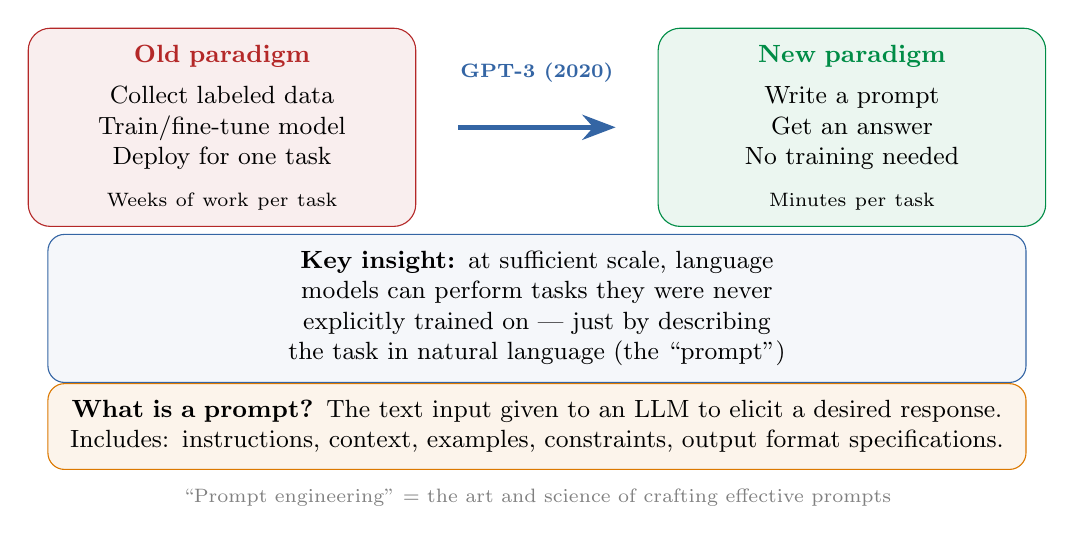
\begin{tikzpicture}
  % Old paradigm
  \node[draw=warnred, fill=warnred!8, rounded corners=8pt, text width=4.5cm, minimum height=2.5cm, align=center, inner sep=6pt, font=\small] at (-4, 1.5) {
    \textbf{\textcolor{warnred}{Old paradigm}}\\[4pt]
    Collect labeled data\\Train/fine-tune model\\Deploy for one task\\[4pt]
    {\scriptsize Weeks of work per task}
  };

  \draw[-Stealth, very thick, popblue, line width=2pt] (-1, 1.5) -- (1, 1.5);
  \node[font=\scriptsize\bfseries, text=popblue] at (0, 2.2) {GPT-3 (2020)};

  % New paradigm
  \node[draw=paramgreen, fill=paramgreen!8, rounded corners=8pt, text width=4.5cm, minimum height=2.5cm, align=center, inner sep=6pt, font=\small] at (4, 1.5) {
    \textbf{\textcolor{paramgreen}{New paradigm}}\\[4pt]
    Write a prompt\\Get an answer\\No training needed\\[4pt]
    {\scriptsize Minutes per task}
  };

  % The key insight
  \node[draw=popblue, fill=popblue!5, rounded corners=6pt, text width=12cm, align=center, inner sep=6pt, font=\small] at (0, -0.8) {
    \textbf{Key insight:} at sufficient scale, language models can perform tasks they were never\\
    explicitly trained on --- just by describing the task in natural language (the ``prompt'')
  };

  % What is a prompt
  \node[draw=orange1, fill=orange1!8, rounded corners=6pt, text width=12cm, align=center, inner sep=6pt, font=\small] at (0, -2.3) {
    \textbf{What is a prompt?} The text input given to an LLM to elicit a desired response.\\
    Includes: instructions, context, examples, constraints, output format specifications.
  };

  \node[font=\scriptsize, text=gray] at (0, -3.2) {
    ``Prompt engineering'' = the art and science of crafting effective prompts
  };
\end{tikzpicture}
\end{center}
\end{frame}

% ============================================================
% ZERO-SHOT PROMPTING
% ============================================================
\begin{frame}
\frametitle{Zero-shot prompting}

\begin{center}
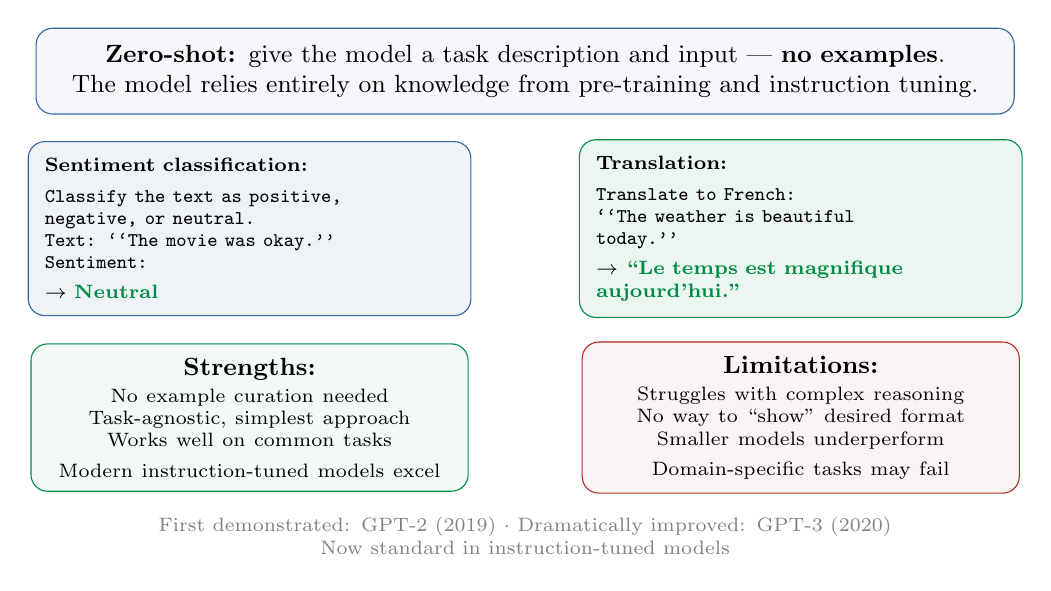
\begin{tikzpicture}
  % Definition
  \node[draw=popblue, fill=popblue!5, rounded corners=6pt, text width=12cm, align=center, inner sep=6pt, font=\small] at (0, 3) {
    \textbf{Zero-shot:} give the model a task description and input --- \textbf{no examples}.\\
    The model relies entirely on knowledge from pre-training and instruction tuning.
  };

  % Examples
  \node[draw=popblue, fill=popblue!8, rounded corners=6pt, text width=5.2cm, align=left, inner sep=6pt, font=\scriptsize] at (-3.5, 1) {
    \textbf{Sentiment classification:}\\[3pt]
    \texttt{Classify the text as positive,}\\
    \texttt{negative, or neutral.}\\
    \texttt{Text: ``The movie was okay.''}\\
    \texttt{Sentiment:}\\[3pt]
    $\to$ \textbf{\textcolor{paramgreen}{Neutral}}
  };

  \node[draw=paramgreen, fill=paramgreen!8, rounded corners=6pt, text width=5.2cm, align=left, inner sep=6pt, font=\scriptsize] at (3.5, 1) {
    \textbf{Translation:}\\[3pt]
    \texttt{Translate to French:}\\
    \texttt{``The weather is beautiful}\\
    \texttt{today.''}\\[3pt]
    $\to$ \textbf{\textcolor{paramgreen}{``Le temps est magnifique}}\\
    \textbf{\textcolor{paramgreen}{aujourd'hui.''}}
  };

  % Strengths and limitations
  \node[draw=paramgreen, fill=paramgreen!5, rounded corners=6pt, text width=5.2cm, align=center, inner sep=5pt, font=\small] at (-3.5, -1.4) {
    \textbf{Strengths:}\\[2pt]
    {\scriptsize No example curation needed\\Task-agnostic, simplest approach\\Works well on common tasks\\Modern instruction-tuned models excel}
  };

  \node[draw=warnred, fill=warnred!5, rounded corners=6pt, text width=5.2cm, align=center, inner sep=5pt, font=\small] at (3.5, -1.4) {
    \textbf{Limitations:}\\[2pt]
    {\scriptsize Struggles with complex reasoning\\No way to ``show'' desired format\\Smaller models underperform\\Domain-specific tasks may fail}
  };

  \node[font=\scriptsize, text=gray, text width=12cm, align=center] at (0, -2.9) {
    First demonstrated: GPT-2 (2019) $\cdot$ Dramatically improved: GPT-3 (2020)\\Now standard in instruction-tuned models
  };
\end{tikzpicture}
\end{center}
\end{frame}

% ============================================================
% FEW-SHOT PROMPTING
% ============================================================
\begin{frame}
\frametitle{Few-shot prompting (in-context learning)}

\begin{center}
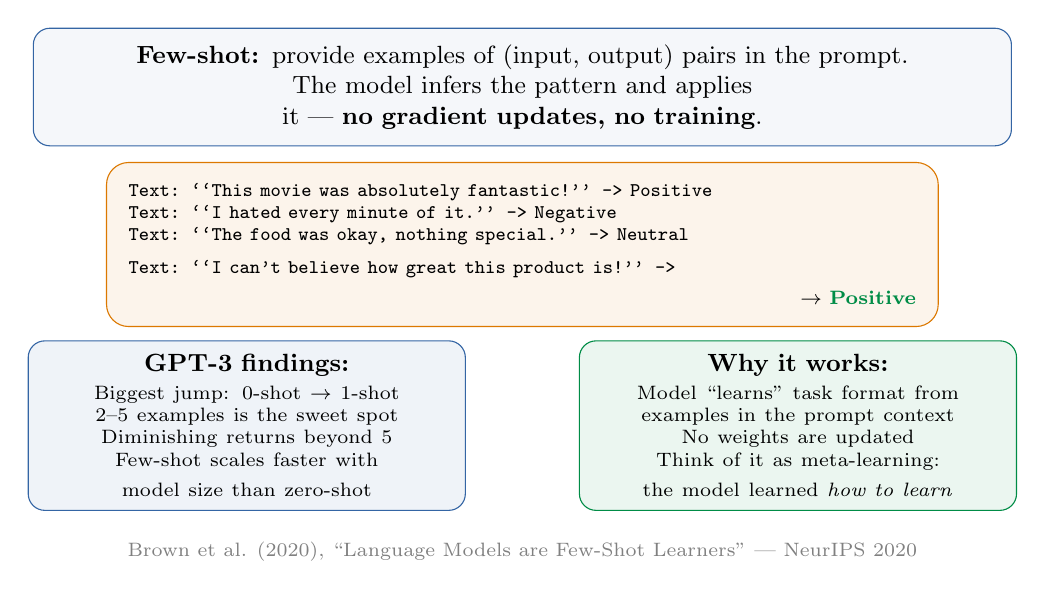
\begin{tikzpicture}
  % Definition
  \node[draw=popblue, fill=popblue!5, rounded corners=6pt, text width=12cm, align=center, inner sep=6pt, font=\small] at (0, 3) {
    \textbf{Few-shot:} provide examples of (input, output) pairs in the prompt.\\
    The model infers the pattern and applies it --- \textbf{no gradient updates, no training}.
  };

  % Concrete example
  \node[draw=orange1, fill=orange1!8, rounded corners=8pt, text width=10cm, align=left, inner sep=8pt, font=\scriptsize] at (0, 1) {
    \texttt{Text: ``This movie was absolutely fantastic!'' -> Positive}\\
    \texttt{Text: ``I hated every minute of it.'' -> Negative}\\
    \texttt{Text: ``The food was okay, nothing special.'' -> Neutral}\\[4pt]
    \texttt{Text: ``I can't believe how great this product is!'' ->}\\[3pt]
    \hfill$\to$ \textbf{\textcolor{paramgreen}{Positive}}
  };

  % Key findings
  \node[draw=popblue, fill=popblue!8, rounded corners=6pt, text width=5.2cm, align=center, inner sep=5pt, font=\small] at (-3.5, -1.3) {
    \textbf{GPT-3 findings:}\\[2pt]
    {\scriptsize Biggest jump: 0-shot $\to$ 1-shot\\2--5 examples is the sweet spot\\Diminishing returns beyond 5\\Few-shot scales faster with\\model size than zero-shot}
  };

  \node[draw=paramgreen, fill=paramgreen!8, rounded corners=6pt, text width=5.2cm, align=center, inner sep=5pt, font=\small] at (3.5, -1.3) {
    \textbf{Why it works:}\\[2pt]
    {\scriptsize Model ``learns'' task format from\\examples in the prompt context\\No weights are updated\\Think of it as meta-learning:\\the model learned \emph{how to learn}}
  };

  \node[font=\scriptsize, text=gray] at (0, -2.9) {
    Brown et al. (2020), ``Language Models are Few-Shot Learners'' --- NeurIPS 2020
  };
\end{tikzpicture}
\end{center}
\end{frame}

% ============================================================
% FEW-SHOT SENSITIVITY
% ============================================================
\begin{frame}
\frametitle{Few-shot is surprisingly fragile}

\begin{center}
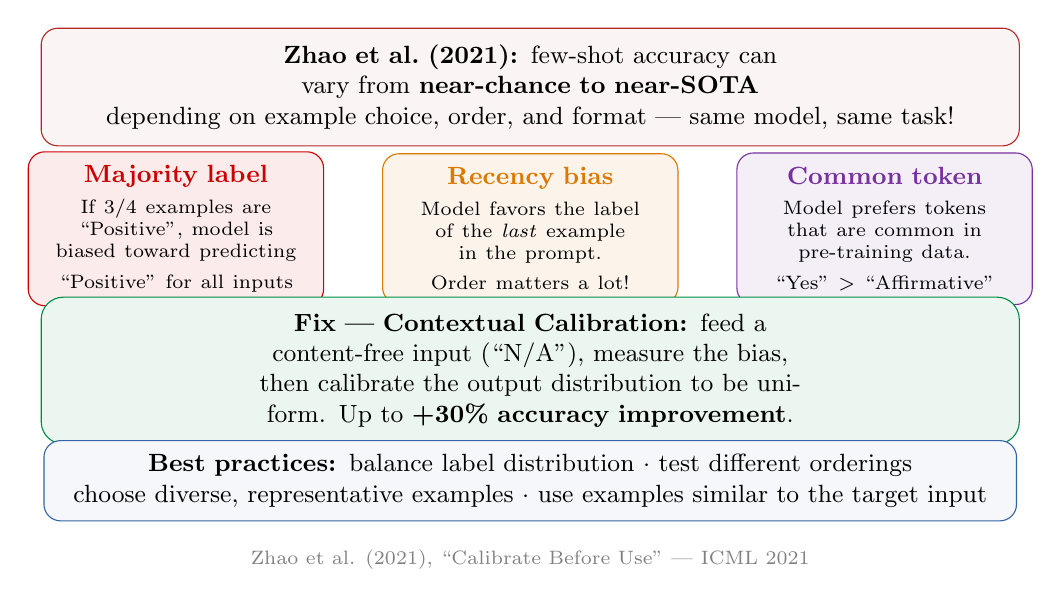
\begin{tikzpicture}
  \node[draw=warnred, fill=warnred!5, rounded corners=6pt, text width=12cm, align=center, inner sep=6pt, font=\small] at (0, 3) {
    \textbf{Zhao et al.\ (2021):} few-shot accuracy can vary from \textbf{near-chance to near-SOTA}\\
    depending on example choice, order, and format --- same model, same task!
  };

  % Three biases
  \node[draw=sampred, fill=sampred!8, rounded corners=6pt, text width=3.4cm, align=center, inner sep=5pt, font=\small] at (-4.5, 1.2) {
    \textbf{\textcolor{sampred}{Majority label}}\\[3pt]
    {\scriptsize If 3/4 examples are\\``Positive'', model is\\biased toward predicting\\``Positive'' for all inputs}
  };

  \node[draw=orange1, fill=orange1!8, rounded corners=6pt, text width=3.4cm, align=center, inner sep=5pt, font=\small] at (0, 1.2) {
    \textbf{\textcolor{orange1}{Recency bias}}\\[3pt]
    {\scriptsize Model favors the label\\of the \emph{last} example\\in the prompt.\\Order matters a lot!}
  };

  \node[draw=violet1, fill=violet1!8, rounded corners=6pt, text width=3.4cm, align=center, inner sep=5pt, font=\small] at (4.5, 1.2) {
    \textbf{\textcolor{violet1}{Common token}}\\[3pt]
    {\scriptsize Model prefers tokens\\that are common in\\pre-training data.\\``Yes'' $>$ ``Affirmative''}
  };

  % Fix
  \node[draw=paramgreen, fill=paramgreen!8, rounded corners=8pt, text width=12cm, align=center, inner sep=6pt, font=\small] at (0, -0.6) {
    \textbf{Fix --- Contextual Calibration:} feed a content-free input (``N/A''), measure the bias,\\
    then calibrate the output distribution to be uniform. Up to \textbf{+30\% accuracy improvement}.
  };

  % Practical tips
  \node[draw=popblue, fill=popblue!5, rounded corners=6pt, text width=12cm, align=center, inner sep=5pt, font=\small] at (0, -2) {
    \textbf{Best practices:} balance label distribution $\cdot$ test different orderings\\
    choose diverse, representative examples $\cdot$ use examples similar to the target input
  };

  \node[font=\scriptsize, text=gray] at (0, -3) {
    Zhao et al. (2021), ``Calibrate Before Use'' --- ICML 2021
  };
\end{tikzpicture}
\end{center}
\end{frame}

% ============================================================
% CHAIN-OF-THOUGHT: FEW-SHOT
% ============================================================
\begin{frame}
\frametitle{Chain-of-Thought prompting (Wei et al., 2022)}

\begin{center}
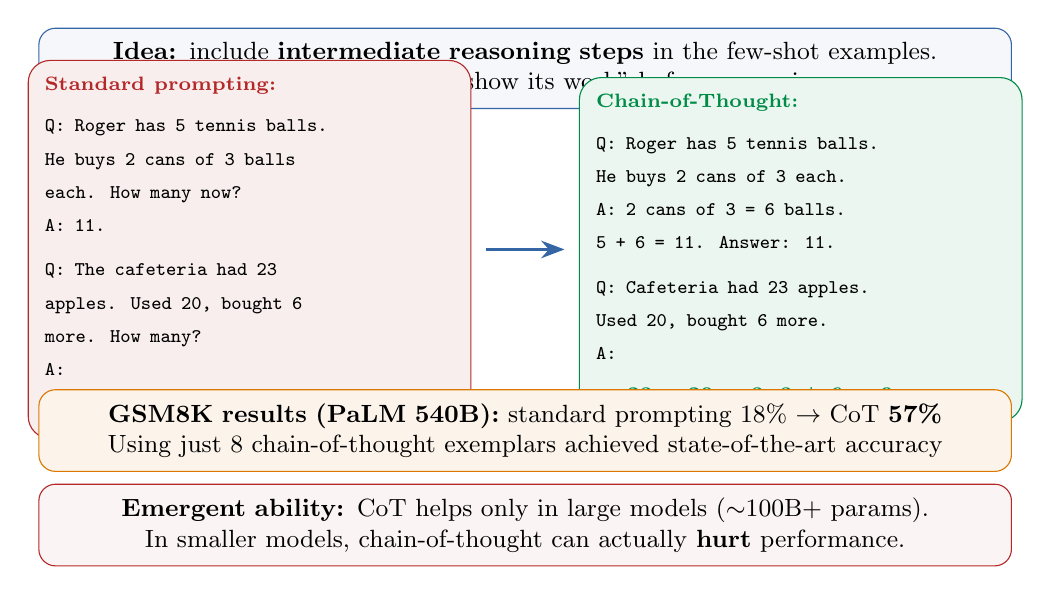
\begin{tikzpicture}
  % The idea
  \node[draw=popblue, fill=popblue!5, rounded corners=6pt, text width=12cm, align=center, inner sep=5pt, font=\small] at (0, 3.1) {
    \textbf{Idea:} include \textbf{intermediate reasoning steps} in the few-shot examples.\\
    The model learns to ``show its work'' before answering.
  };

  % Without CoT
  \node[draw=warnred, fill=warnred!8, rounded corners=8pt, text width=5.2cm, align=left, inner sep=6pt] at (-3.5, 0.8) {
    {\scriptsize\bfseries\textcolor{warnred}{Standard prompting:}}\\[3pt]
    {\scriptsize\texttt{Q: Roger has 5 tennis balls.}}\\
    {\scriptsize\texttt{He buys 2 cans of 3 balls}}\\
    {\scriptsize\texttt{each. How many now?}}\\
    {\scriptsize\texttt{A: 11.}}\\[4pt]
    {\scriptsize\texttt{Q: The cafeteria had 23}}\\
    {\scriptsize\texttt{apples. Used 20, bought 6}}\\
    {\scriptsize\texttt{more. How many?}}\\
    {\scriptsize\texttt{A:}}\\[3pt]
    {\scriptsize $\to$ \textcolor{warnred}{\textbf{27}} \quad (wrong!)}
  };

  % With CoT
  \node[draw=paramgreen, fill=paramgreen!8, rounded corners=8pt, text width=5.2cm, align=left, inner sep=6pt] at (3.5, 0.8) {
    {\scriptsize\bfseries\textcolor{paramgreen}{Chain-of-Thought:}}\\[3pt]
    {\scriptsize\texttt{Q: Roger has 5 tennis balls.}}\\
    {\scriptsize\texttt{He buys 2 cans of 3 each.}}\\
    {\scriptsize\texttt{A: 2 cans of 3 = 6 balls.}}\\
    {\scriptsize\texttt{5 + 6 = 11. Answer: 11.}}\\[4pt]
    {\scriptsize\texttt{Q: Cafeteria had 23 apples.}}\\
    {\scriptsize\texttt{Used 20, bought 6 more.}}\\
    {\scriptsize\texttt{A:}}\\[3pt]
    {\scriptsize $\to$ \textcolor{paramgreen}{\textbf{23 $-$ 20 = 3, 3 + 6 = 9.}}}
  };

  % Arrow
  \draw[-Stealth, very thick, popblue] (-0.5, 0.8) -- (0.5, 0.8);

  % Results
  \node[draw=orange1, fill=orange1!8, rounded corners=6pt, text width=12cm, align=center, inner sep=5pt, font=\small] at (0, -1.5) {
    \textbf{GSM8K results (PaLM 540B):} standard prompting 18\% $\to$ CoT \textbf{57\%}\\
    Using just 8 chain-of-thought exemplars achieved state-of-the-art accuracy
  };

  % Emergent
  \node[draw=warnred, fill=warnred!5, rounded corners=6pt, text width=12cm, align=center, inner sep=5pt, font=\small] at (0, -2.7) {
    \textbf{Emergent ability:} CoT helps only in large models ($\sim$100B+ params).\\
    In smaller models, chain-of-thought can actually \textbf{hurt} performance.
  };
\end{tikzpicture}
\end{center}
\end{frame}

% ============================================================
% ZERO-SHOT COT
% ============================================================
\begin{frame}
\frametitle{Zero-shot CoT: ``Let's think step by step''}

\begin{center}
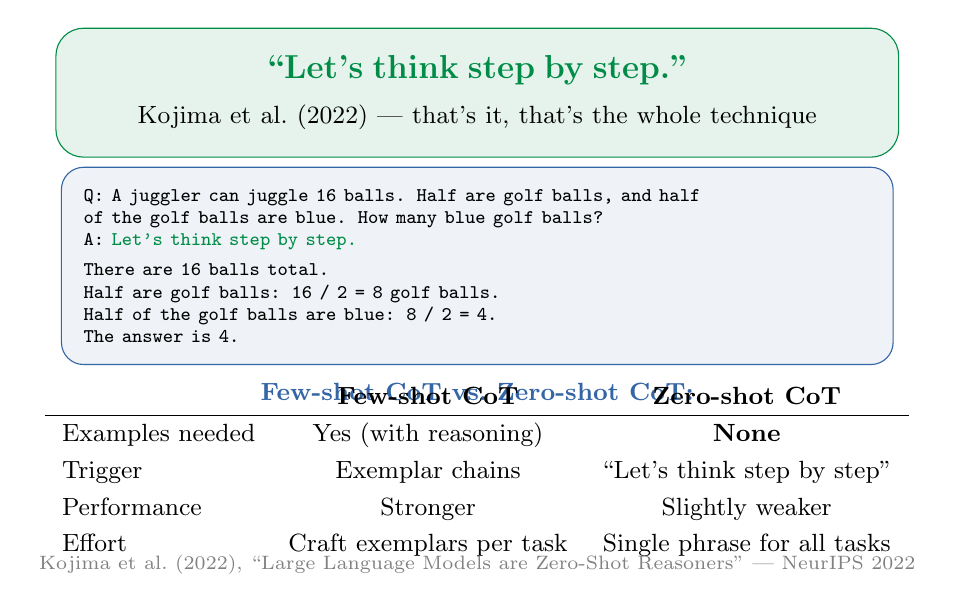
\begin{tikzpicture}
  % The magic phrase
  \node[draw=paramgreen, fill=paramgreen!10, rounded corners=10pt, text width=10cm, align=center, inner sep=10pt] at (0, 3) {
    {\large\bfseries\textcolor{paramgreen}{``Let's think step by step.''}}\\[4pt]
    {\small Kojima et al.\ (2022) --- that's it, that's the whole technique}
  };

  % Example
  \node[draw=popblue, fill=popblue!8, rounded corners=8pt, text width=10cm, align=left, inner sep=8pt, font=\scriptsize] at (0, 0.8) {
    \texttt{Q: A juggler can juggle 16 balls. Half are golf balls, and half}\\
    \texttt{of the golf balls are blue. How many blue golf balls?}\\
    \texttt{A: \textcolor{paramgreen}{\textbf{Let's think step by step.}}}\\[3pt]
    \texttt{There are 16 balls total.}\\
    \texttt{Half are golf balls: 16 / 2 = 8 golf balls.}\\
    \texttt{Half of the golf balls are blue: 8 / 2 = 4.}\\
    \texttt{\textbf{The answer is 4.}}
  };

  % Comparison table
  \node[font=\small\bfseries, text=popblue] at (0, -0.8) {Few-shot CoT vs.\ Zero-shot CoT:};

  \node at (0, -1.8) {
    {\small
    \renewcommand{\arraystretch}{1.2}
    \begin{tabular}{l c c}
      & \textbf{Few-shot CoT} & \textbf{Zero-shot CoT} \\
      \hline
      Examples needed & Yes (with reasoning) & \textbf{None} \\
      Trigger & Exemplar chains & ``Let's think step by step'' \\
      Performance & Stronger & Slightly weaker \\
      Effort & Craft exemplars per task & Single phrase for all tasks \\
    \end{tabular}
    }
  };

  \node[font=\scriptsize, text=gray] at (0, -3) {
    Kojima et al.\ (2022), ``Large Language Models are Zero-Shot Reasoners'' --- NeurIPS 2022
  };
\end{tikzpicture}
\end{center}
\end{frame}

% ============================================================
% WHY COT WORKS
% ============================================================
\begin{frame}
\frametitle{Why does Chain-of-Thought work?}

\begin{center}
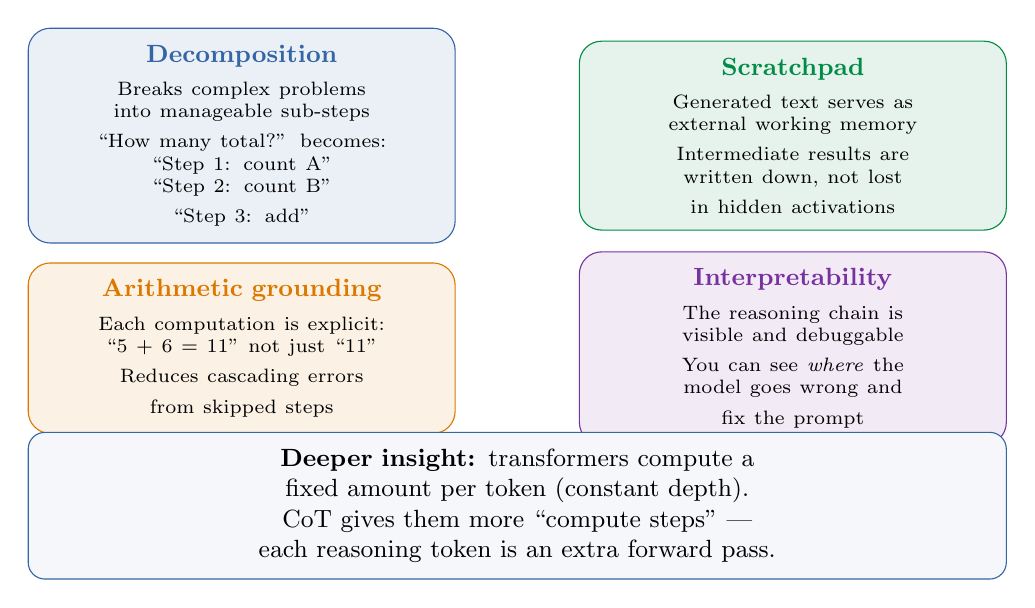
\begin{tikzpicture}
  % Four reasons
  \node[draw=popblue, fill=popblue!10, rounded corners=8pt, text width=5cm, align=center, inner sep=6pt, font=\small] at (-3.5, 2.2) {
    \textbf{\textcolor{popblue}{Decomposition}}\\[4pt]
    {\scriptsize Breaks complex problems\\into manageable sub-steps\\[3pt]
    ``How many total?'' becomes:\\``Step 1: count A''\\``Step 2: count B''\\``Step 3: add''}
  };

  \node[draw=paramgreen, fill=paramgreen!10, rounded corners=8pt, text width=5cm, align=center, inner sep=6pt, font=\small] at (3.5, 2.2) {
    \textbf{\textcolor{paramgreen}{Scratchpad}}\\[4pt]
    {\scriptsize Generated text serves as\\external working memory\\[3pt]
    Intermediate results are\\written down, not lost\\in hidden activations}
  };

  \node[draw=orange1, fill=orange1!10, rounded corners=8pt, text width=5cm, align=center, inner sep=6pt, font=\small] at (-3.5, -0.5) {
    \textbf{\textcolor{orange1}{Arithmetic grounding}}\\[4pt]
    {\scriptsize Each computation is explicit:\\``5 + 6 = 11'' not just ``11''\\[3pt]
    Reduces cascading errors\\from skipped steps}
  };

  \node[draw=violet1, fill=violet1!10, rounded corners=8pt, text width=5cm, align=center, inner sep=6pt, font=\small] at (3.5, -0.5) {
    \textbf{\textcolor{violet1}{Interpretability}}\\[4pt]
    {\scriptsize The reasoning chain is\\visible and debuggable\\[3pt]
    You can see \emph{where} the\\model goes wrong and\\fix the prompt}
  };

  % Bottom insight
  \node[draw=popblue, fill=popblue!5, rounded corners=6pt, text width=12cm, align=center, inner sep=6pt, font=\small] at (0, -2.5) {
    \textbf{Deeper insight:} transformers compute a fixed amount per token (constant depth).\\
    CoT gives them more ``compute steps'' --- each reasoning token is an extra forward pass.
  };
\end{tikzpicture}
\end{center}
\end{frame}

% ============================================================
% SELF-CONSISTENCY
% ============================================================
\begin{frame}
\frametitle{Self-Consistency (Wang et al., 2022)}

\begin{center}
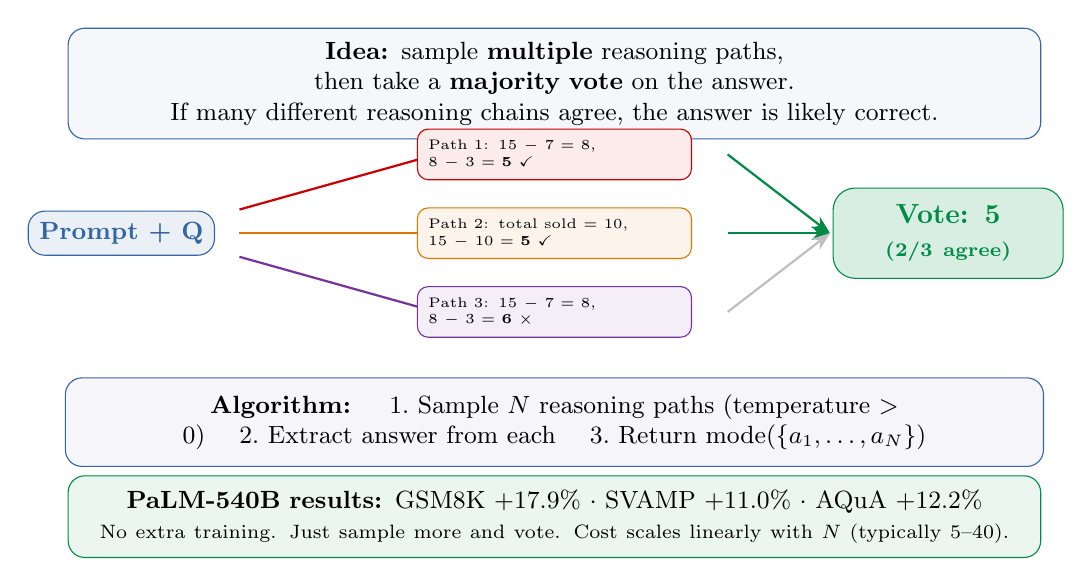
\begin{tikzpicture}
  % The idea
  \node[draw=popblue, fill=popblue!5, rounded corners=6pt, text width=12cm, align=center, inner sep=5pt, font=\small] at (0, 3.1) {
    \textbf{Idea:} sample \textbf{multiple} reasoning paths, then take a \textbf{majority vote} on the answer.\\
    If many different reasoning chains agree, the answer is likely correct.
  };

  % Diagram
  \node[draw=popblue, fill=popblue!10, rounded corners=6pt, inner sep=4pt, font=\small\bfseries, text=popblue] at (-5.5, 1.2) {Prompt + Q};

  % Three paths
  \draw[-Stealth, thick, sampred] (-4, 1.5) -- (-1.5, 2.2);
  \draw[-Stealth, thick, orange1] (-4, 1.2) -- (-1.5, 1.2);
  \draw[-Stealth, thick, violet1] (-4, 0.9) -- (-1.5, 0.2);

  \node[draw=sampred, fill=sampred!8, rounded corners=4pt, text width=3.2cm, align=left, inner sep=4pt, font=\tiny] at (0, 2.2) {
    Path 1: 15 $-$ 7 = 8,\\8 $-$ 3 = \textbf{5} $\checkmark$
  };
  \node[draw=orange1, fill=orange1!8, rounded corners=4pt, text width=3.2cm, align=left, inner sep=4pt, font=\tiny] at (0, 1.2) {
    Path 2: total sold = 10,\\15 $-$ 10 = \textbf{5} $\checkmark$
  };
  \node[draw=violet1, fill=violet1!8, rounded corners=4pt, text width=3.2cm, align=left, inner sep=4pt, font=\tiny] at (0, 0.2) {
    Path 3: 15 $-$ 7 = 8,\\8 $-$ 3 = \textbf{6} $\times$
  };

  % Majority vote
  \draw[-Stealth, thick, paramgreen] (2.2, 2.2) -- (3.5, 1.2);
  \draw[-Stealth, thick, paramgreen] (2.2, 1.2) -- (3.5, 1.2);
  \draw[-Stealth, thick, gray!50] (2.2, 0.2) -- (3.5, 1.2);

  \node[draw=paramgreen, fill=paramgreen!15, rounded corners=8pt, inner sep=6pt, text width=2.5cm, align=center, font=\normalsize\bfseries, text=paramgreen] at (5, 1.2) {
    Vote: \textbf{5}\\{\scriptsize (2/3 agree)}
  };

  % Algorithm
  \node[draw=popblue, fill=lightbg, rounded corners=6pt, text width=12cm, align=center, inner sep=6pt, font=\small] at (0, -1.2) {
    \textbf{Algorithm:} \quad
    1.\ Sample $N$ reasoning paths (temperature $> 0$) \quad
    2.\ Extract answer from each \quad
    3.\ Return $\text{mode}(\{a_1, \ldots, a_N\})$
  };

  % Results
  \node[draw=paramgreen, fill=paramgreen!8, rounded corners=6pt, text width=12cm, align=center, inner sep=5pt, font=\small] at (0, -2.4) {
    \textbf{PaLM-540B results:} GSM8K +17.9\% $\cdot$ SVAMP +11.0\% $\cdot$ AQuA +12.2\%\\
    {\scriptsize No extra training. Just sample more and vote. Cost scales linearly with $N$ (typically 5--40).}
  };
\end{tikzpicture}
\end{center}
\end{frame}

% ============================================================
% TREE OF THOUGHTS
% ============================================================
\begin{frame}
\frametitle{Tree of Thoughts (Yao et al., 2023)}

\begin{center}
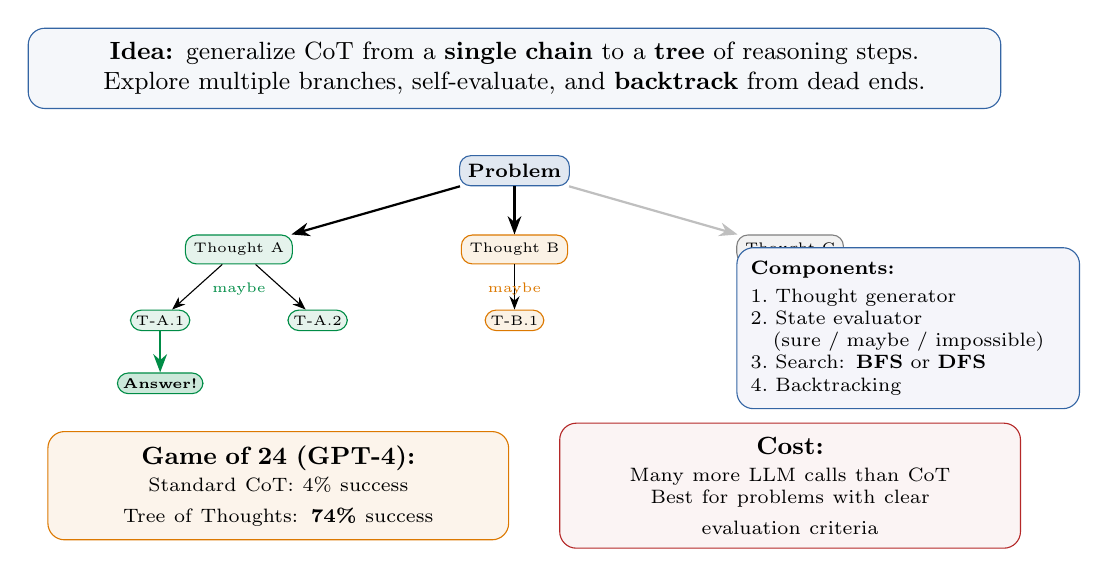
\begin{tikzpicture}
  % Definition
  \node[draw=popblue, fill=popblue!5, rounded corners=6pt, text width=12cm, align=center, inner sep=5pt, font=\small] at (0, 3.1) {
    \textbf{Idea:} generalize CoT from a \textbf{single chain} to a \textbf{tree} of reasoning steps.\\
    Explore multiple branches, self-evaluate, and \textbf{backtrack} from dead ends.
  };

  % Tree diagram
  \node[draw=popblue, fill=popblue!15, rounded corners=4pt, inner sep=3pt, font=\scriptsize\bfseries] (root) at (0, 1.8) {Problem};

  \node[draw=paramgreen, fill=paramgreen!10, rounded corners=4pt, inner sep=3pt, font=\tiny] (t1) at (-3.5, 0.8) {Thought A};
  \node[draw=orange1, fill=orange1!10, rounded corners=4pt, inner sep=3pt, font=\tiny] (t2) at (0, 0.8) {Thought B};
  \node[draw=gray, fill=gray!10, rounded corners=4pt, inner sep=3pt, font=\tiny] (t3) at (3.5, 0.8) {Thought C};

  \draw[-Stealth, thick] (root) -- (t1);
  \draw[-Stealth, thick] (root) -- (t2);
  \draw[-Stealth, thick, gray!50] (root) -- (t3);

  \node[draw=paramgreen, fill=paramgreen!10, rounded corners=4pt, inner sep=2pt, font=\tiny] (t11) at (-4.5, -0.1) {T-A.1};
  \node[draw=paramgreen, fill=paramgreen!10, rounded corners=4pt, inner sep=2pt, font=\tiny] (t12) at (-2.5, -0.1) {T-A.2};
  \node[draw=orange1, fill=orange1!10, rounded corners=4pt, inner sep=2pt, font=\tiny] (t21) at (0, -0.1) {T-B.1};

  \draw[-Stealth] (t1) -- (t11);
  \draw[-Stealth] (t1) -- (t12);
  \draw[-Stealth] (t2) -- (t21);

  \node[draw=paramgreen, fill=paramgreen!20, rounded corners=4pt, inner sep=2pt, font=\tiny\bfseries] (ans) at (-4.5, -0.9) {Answer!};
  \draw[-Stealth, thick, paramgreen] (t11) -- (ans);

  % Labels
  \node[font=\tiny, text=paramgreen] at (-3.5, 0.3) {maybe};
  \node[font=\tiny, text=orange1] at (0, 0.3) {maybe};
  \node[font=\tiny, text=warnred] at (3.5, 0.3) {impossible};
  \node[font=\tiny\bfseries, text=warnred] at (3.5, 0.55) {$\times$ prune};

  % Three components on the right
  \node[draw=popblue, fill=lightbg, rounded corners=6pt, text width=4cm, align=left, inner sep=5pt, font=\scriptsize] at (5, -0.2) {
    \textbf{Components:}\\[2pt]
    1.\ Thought generator\\
    2.\ State evaluator\\
    \quad (sure / maybe / impossible)\\
    3.\ Search: \textbf{BFS} or \textbf{DFS}\\
    4.\ Backtracking
  };

  % Game of 24 example
  \node[draw=orange1, fill=orange1!8, rounded corners=6pt, text width=5.5cm, align=center, inner sep=5pt, font=\small] at (-3, -2.2) {
    \textbf{Game of 24 (GPT-4):}\\[2pt]
    {\scriptsize Standard CoT: 4\% success\\Tree of Thoughts: \textbf{74\%} success}
  };

  \node[draw=warnred, fill=warnred!5, rounded corners=6pt, text width=5.5cm, align=center, inner sep=5pt, font=\small] at (3.5, -2.2) {
    \textbf{Cost:}\\[2pt]
    {\scriptsize Many more LLM calls than CoT\\Best for problems with clear\\evaluation criteria}
  };
\end{tikzpicture}
\end{center}
\end{frame}

% ============================================================
% REACT
% ============================================================
\begin{frame}
\frametitle{ReAct: Reasoning + Acting (Yao et al., 2022)}

\begin{center}
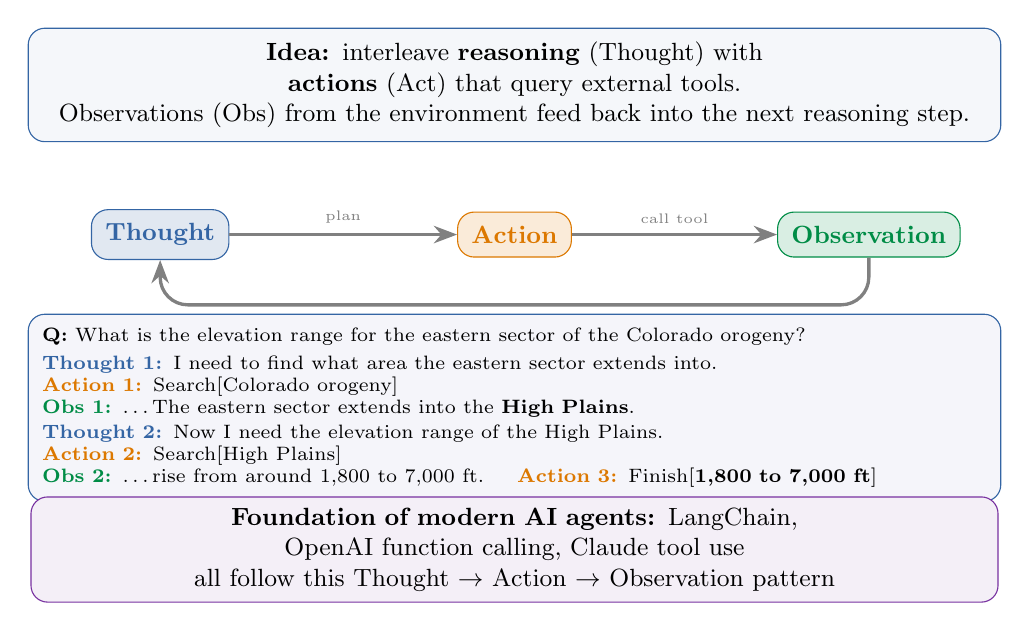
\begin{tikzpicture}
  % Definition
  \node[draw=popblue, fill=popblue!5, rounded corners=6pt, text width=12cm, align=center, inner sep=5pt, font=\small] at (0, 3.1) {
    \textbf{Idea:} interleave \textbf{reasoning} (Thought) with \textbf{actions} (Act) that query external tools.\\
    Observations (Obs) from the environment feed back into the next reasoning step.
  };

  % The loop diagram
  \node[draw=popblue, fill=popblue!15, rounded corners=6pt, inner sep=5pt, font=\small\bfseries, text=popblue] (thought) at (-4.5, 1.2) {Thought};
  \node[draw=orange1, fill=orange1!15, rounded corners=6pt, inner sep=5pt, font=\small\bfseries, text=orange1] (action) at (0, 1.2) {Action};
  \node[draw=paramgreen, fill=paramgreen!15, rounded corners=6pt, inner sep=5pt, font=\small\bfseries, text=paramgreen] (obs) at (4.5, 1.2) {Observation};

  \draw[-Stealth, very thick, gray] (thought) -- node[above, font=\tiny] {plan} (action);
  \draw[-Stealth, very thick, gray] (action) -- node[above, font=\tiny] {call tool} (obs);
  \draw[-Stealth, very thick, gray, rounded corners=10pt] (obs.south) -- ++(0, -0.6) -| (thought.south);

  % Example
  \node[draw=popblue, fill=lightbg, rounded corners=6pt, text width=12cm, align=left, inner sep=5pt, font=\scriptsize] at (0, -1) {
    \textbf{Q:} What is the elevation range for the eastern sector of the Colorado orogeny?\\[2pt]
    \textcolor{popblue}{\textbf{Thought 1:}} I need to find what area the eastern sector extends into.\\
    \textcolor{orange1}{\textbf{Action 1:}} Search[Colorado orogeny]\\
    \textcolor{paramgreen}{\textbf{Obs 1:}} \ldots The eastern sector extends into the \textbf{High Plains}.\\[1pt]
    \textcolor{popblue}{\textbf{Thought 2:}} Now I need the elevation range of the High Plains.\\
    \textcolor{orange1}{\textbf{Action 2:}} Search[High Plains]\\
    \textcolor{paramgreen}{\textbf{Obs 2:}} \ldots rise from around 1,800 to 7,000 ft. \quad
    \textcolor{orange1}{\textbf{Action 3:}} Finish[\textbf{1,800 to 7,000 ft}]
  };

  % Why it matters
  \node[draw=violet1, fill=violet1!8, rounded corners=6pt, text width=12cm, align=center, inner sep=4pt, font=\small] at (0, -2.8) {
    \textbf{Foundation of modern AI agents:} LangChain, OpenAI function calling, Claude tool use\\
    all follow this Thought $\to$ Action $\to$ Observation pattern
  };
\end{tikzpicture}
\end{center}
\end{frame}

% ============================================================
% REACT: WHY BOTH MATTER
% ============================================================
\begin{frame}
\frametitle{ReAct: why reasoning AND acting both matter}

\begin{center}
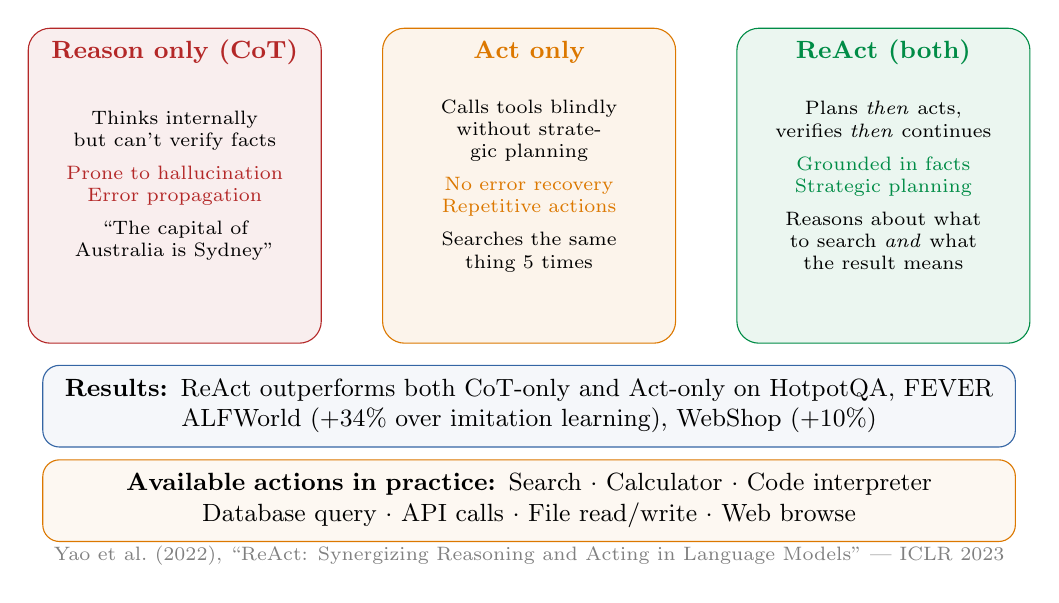
\begin{tikzpicture}
  % Three approaches
  \node[draw=warnred, fill=warnred!8, rounded corners=8pt, text width=3.3cm, minimum height=4cm, align=center, inner sep=6pt] at (-4.5, 1.5) {};
  \node[font=\small\bfseries, text=warnred] at (-4.5, 3.2) {Reason only (CoT)};
  \node[font=\scriptsize, text width=3cm, align=center] at (-4.5, 1.5) {
    Thinks internally\\but can't verify facts\\[4pt]
    \textcolor{warnred}{Prone to hallucination}\\
    \textcolor{warnred}{Error propagation}\\[4pt]
    ``The capital of\\Australia is Sydney''
  };

  \node[draw=orange1, fill=orange1!8, rounded corners=8pt, text width=3.3cm, minimum height=4cm, align=center, inner sep=6pt] at (0, 1.5) {};
  \node[font=\small\bfseries, text=orange1] at (0, 3.2) {Act only};
  \node[font=\scriptsize, text width=3cm, align=center] at (0, 1.5) {
    Calls tools blindly\\without strategic planning\\[4pt]
    \textcolor{orange1}{No error recovery}\\
    \textcolor{orange1}{Repetitive actions}\\[4pt]
    Searches the same\\thing 5 times
  };

  \node[draw=paramgreen, fill=paramgreen!8, rounded corners=8pt, text width=3.3cm, minimum height=4cm, align=center, inner sep=6pt] at (4.5, 1.5) {};
  \node[font=\small\bfseries, text=paramgreen] at (4.5, 3.2) {ReAct (both)};
  \node[font=\scriptsize, text width=3cm, align=center] at (4.5, 1.5) {
    Plans \emph{then} acts,\\verifies \emph{then} continues\\[4pt]
    \textcolor{paramgreen}{Grounded in facts}\\
    \textcolor{paramgreen}{Strategic planning}\\[4pt]
    Reasons about what\\to search \emph{and} what\\the result means
  };

  % Results
  \node[draw=popblue, fill=popblue!5, rounded corners=6pt, text width=12cm, align=center, inner sep=5pt, font=\small] at (0, -1.3) {
    \textbf{Results:} ReAct outperforms both CoT-only and Act-only on HotpotQA, FEVER\\
    ALFWorld (+34\% over imitation learning), WebShop (+10\%)
  };

  % Modern agents
  \node[draw=orange1, fill=orange1!5, rounded corners=6pt, text width=12cm, align=center, inner sep=5pt, font=\small] at (0, -2.5) {
    \textbf{Available actions in practice:} Search $\cdot$ Calculator $\cdot$ Code interpreter\\
    Database query $\cdot$ API calls $\cdot$ File read/write $\cdot$ Web browse
  };

  \node[font=\scriptsize, text=gray] at (0, -3.2) {
    Yao et al.\ (2022), ``ReAct: Synergizing Reasoning and Acting in Language Models'' --- ICLR 2023
  };
\end{tikzpicture}
\end{center}
\end{frame}

% ============================================================
% PROMPT ENGINEERING BEST PRACTICES
% ============================================================
\begin{frame}
\frametitle{Prompt engineering: best practices}

\begin{center}
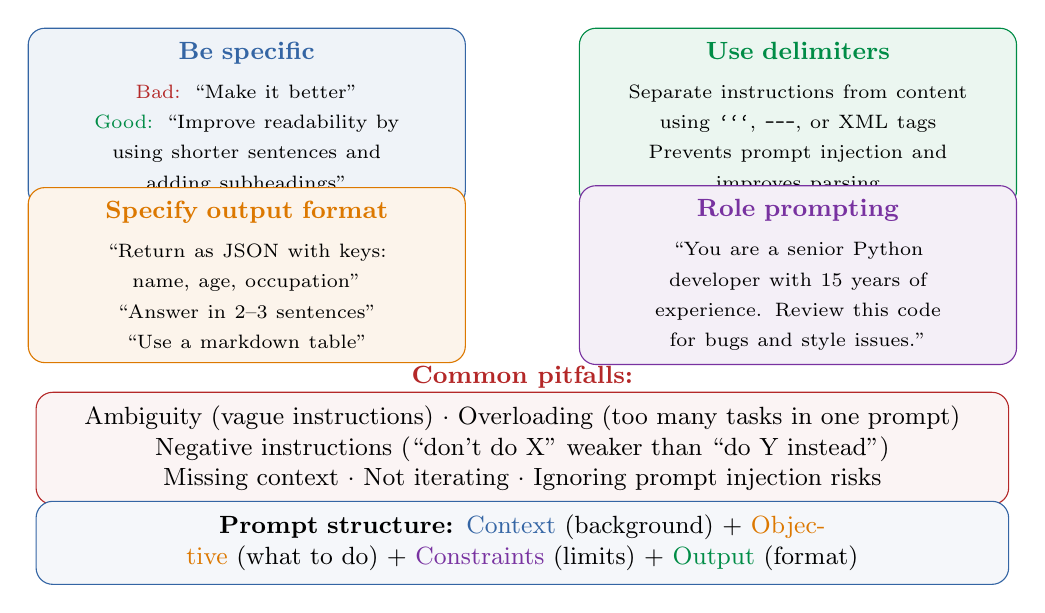
\begin{tikzpicture}
  % Be specific
  \node[draw=popblue, fill=popblue!8, rounded corners=6pt, text width=5.2cm, align=center, inner sep=5pt, font=\small] at (-3.5, 2.5) {
    \textbf{\textcolor{popblue}{Be specific}}\\[3pt]
    {\scriptsize \textcolor{warnred}{Bad:} ``Make it better''}\\
    {\scriptsize \textcolor{paramgreen}{Good:} ``Improve readability by}\\
    {\scriptsize using shorter sentences and}\\
    {\scriptsize adding subheadings''}
  };

  % Use delimiters
  \node[draw=paramgreen, fill=paramgreen!8, rounded corners=6pt, text width=5.2cm, align=center, inner sep=5pt, font=\small] at (3.5, 2.5) {
    \textbf{\textcolor{paramgreen}{Use delimiters}}\\[3pt]
    {\scriptsize Separate instructions from content}\\
    {\scriptsize using \texttt{```}, \texttt{---}, or XML tags}\\
    {\scriptsize Prevents prompt injection and}\\
    {\scriptsize improves parsing}
  };

  % Specify format
  \node[draw=orange1, fill=orange1!8, rounded corners=6pt, text width=5.2cm, align=center, inner sep=5pt, font=\small] at (-3.5, 0.5) {
    \textbf{\textcolor{orange1}{Specify output format}}\\[3pt]
    {\scriptsize ``Return as JSON with keys:}\\
    {\scriptsize name, age, occupation''}\\
    {\scriptsize ``Answer in 2--3 sentences''}\\
    {\scriptsize ``Use a markdown table''}
  };

  % Give role
  \node[draw=violet1, fill=violet1!8, rounded corners=6pt, text width=5.2cm, align=center, inner sep=5pt, font=\small] at (3.5, 0.5) {
    \textbf{\textcolor{violet1}{Role prompting}}\\[3pt]
    {\scriptsize ``You are a senior Python}\\
    {\scriptsize developer with 15 years of}\\
    {\scriptsize experience. Review this code}\\
    {\scriptsize for bugs and style issues.''}
  };

  % Common pitfalls
  \node[font=\small\bfseries, text=warnred] at (0, -0.8) {Common pitfalls:};

  \node[draw=warnred, fill=warnred!5, rounded corners=6pt, text width=12cm, align=center, inner sep=5pt, font=\small] at (0, -1.7) {
    Ambiguity (vague instructions) $\cdot$ Overloading (too many tasks in one prompt)\\
    Negative instructions (``don't do X'' weaker than ``do Y instead'')\\
    Missing context $\cdot$ Not iterating $\cdot$ Ignoring prompt injection risks
  };

  % COCO framework
  \node[draw=popblue, fill=popblue!5, rounded corners=6pt, text width=12cm, align=center, inner sep=5pt, font=\small] at (0, -2.9) {
    \textbf{Prompt structure:} \textcolor{popblue}{Context} (background) + \textcolor{orange1}{Objective} (what to do) + \textcolor{violet1}{Constraints} (limits) + \textcolor{paramgreen}{Output} (format)
  };
\end{tikzpicture}
\end{center}
\end{frame}

% ============================================================
% SYSTEM PROMPTS AND TEMPERATURE
% ============================================================
\begin{frame}
\frametitle{System prompts and temperature}

\begin{center}
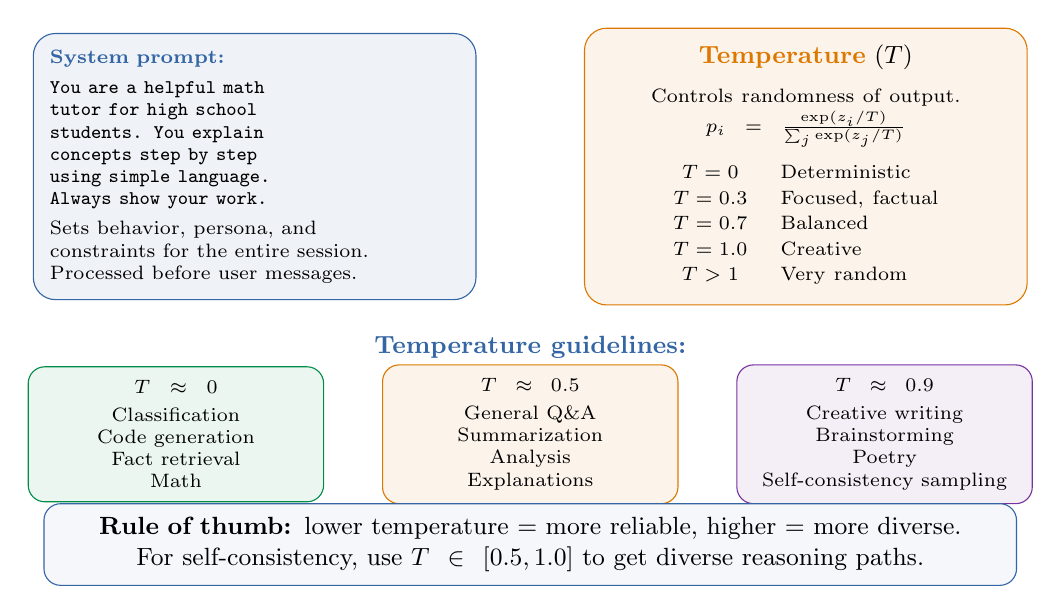
\begin{tikzpicture}
  % System prompt
  \node[draw=popblue, fill=popblue!8, rounded corners=8pt, text width=5.2cm, align=left, inner sep=6pt, font=\scriptsize] at (-3.5, 2) {
    \textbf{\textcolor{popblue}{System prompt:}}\\[3pt]
    \texttt{You are a helpful math}\\
    \texttt{tutor for high school}\\
    \texttt{students. You explain}\\
    \texttt{concepts step by step}\\
    \texttt{using simple language.}\\
    \texttt{Always show your work.}\\[3pt]
    {\scriptsize Sets behavior, persona, and\\constraints for the entire session.\\Processed before user messages.}
  };

  % Temperature
  \node[draw=orange1, fill=orange1!8, rounded corners=8pt, text width=5.2cm, align=center, inner sep=6pt, font=\small] at (3.5, 2) {
    \textbf{\textcolor{orange1}{Temperature}} ($T$)\\[3pt]
    {\scriptsize Controls randomness of output.}\\
    {\scriptsize $p_i = \frac{\exp(z_i / T)}{\sum_j \exp(z_j / T)}$}\\[4pt]
    {\scriptsize
    \renewcommand{\arraystretch}{1.15}
    \begin{tabular}{c l}
      $T = 0$ & Deterministic \\
      $T = 0.3$ & Focused, factual \\
      $T = 0.7$ & Balanced \\
      $T = 1.0$ & Creative \\
      $T > 1$ & Very random \\
    \end{tabular}
    }
  };

  % When to use what
  \node[font=\small\bfseries, text=popblue] at (0, -0.3) {Temperature guidelines:};

  \node[draw=paramgreen, fill=paramgreen!8, rounded corners=6pt, text width=3.4cm, align=center, inner sep=5pt, font=\scriptsize] at (-4.5, -1.4) {
    \textbf{$T \approx 0$}\\[2pt]
    Classification\\Code generation\\Fact retrieval\\Math
  };

  \node[draw=orange1, fill=orange1!8, rounded corners=6pt, text width=3.4cm, align=center, inner sep=5pt, font=\scriptsize] at (0, -1.4) {
    \textbf{$T \approx 0.5$}\\[2pt]
    General Q\&A\\Summarization\\Analysis\\Explanations
  };

  \node[draw=violet1, fill=violet1!8, rounded corners=6pt, text width=3.4cm, align=center, inner sep=5pt, font=\scriptsize] at (4.5, -1.4) {
    \textbf{$T \approx 0.9$}\\[2pt]
    Creative writing\\Brainstorming\\Poetry\\Self-consistency sampling
  };

  \node[draw=popblue, fill=popblue!5, rounded corners=6pt, text width=12cm, align=center, inner sep=5pt, font=\small] at (0, -2.8) {
    \textbf{Rule of thumb:} lower temperature = more reliable, higher = more diverse.\\
    For self-consistency, use $T \in [0.5, 1.0]$ to get diverse reasoning paths.
  };
\end{tikzpicture}
\end{center}
\end{frame}

% ============================================================
% STRUCTURED OUTPUT
% ============================================================
\begin{frame}
\frametitle{Structured output prompting}

\begin{center}
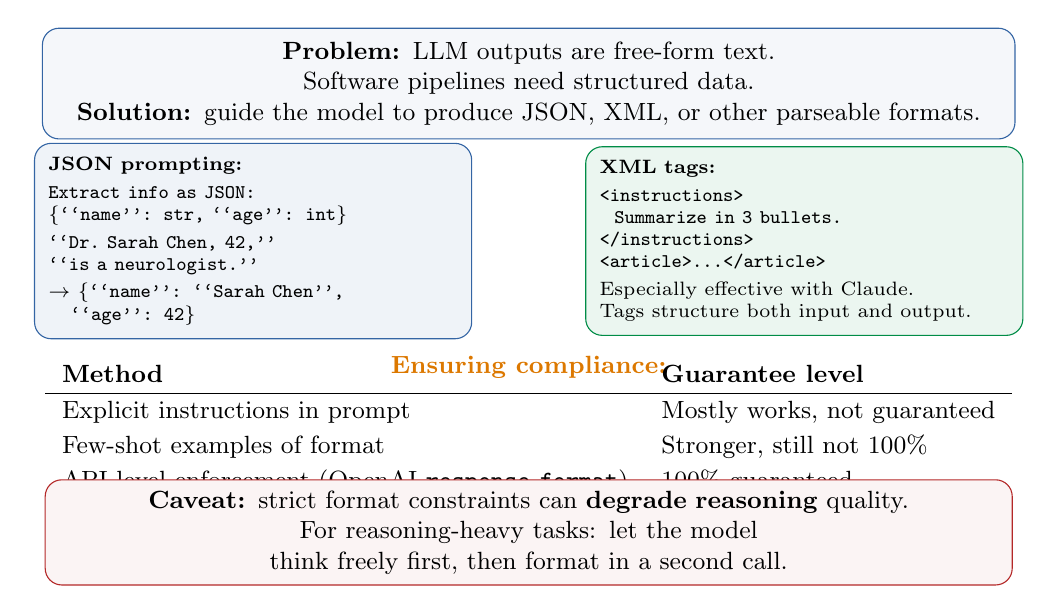
\begin{tikzpicture}
  % Why
  \node[draw=popblue, fill=popblue!5, rounded corners=6pt, text width=12cm, align=center, inner sep=5pt, font=\small] at (0, 3.1) {
    \textbf{Problem:} LLM outputs are free-form text. Software pipelines need structured data.\\
    \textbf{Solution:} guide the model to produce JSON, XML, or other parseable formats.
  };

  % JSON example
  \node[draw=popblue, fill=popblue!8, rounded corners=6pt, text width=5.2cm, align=left, inner sep=5pt, font=\scriptsize] at (-3.5, 1.1) {
    \textbf{JSON prompting:}\\[2pt]
    \texttt{Extract info as JSON:}\\
    \texttt{\{``name'': str, ``age'': int\}}\\[2pt]
    \texttt{``Dr.\ Sarah Chen, 42,''}\\
    \texttt{``is a neurologist.''}\\[2pt]
    $\to$ \texttt{\{``name'': ``Sarah Chen'',}\\
    \quad\texttt{``age'': 42\}}
  };

  % XML example
  \node[draw=paramgreen, fill=paramgreen!8, rounded corners=6pt, text width=5.2cm, align=left, inner sep=5pt, font=\scriptsize] at (3.5, 1.1) {
    \textbf{XML tags:}\\[2pt]
    \texttt{<instructions>}\\
    \texttt{\ \ Summarize in 3 bullets.}\\
    \texttt{</instructions>}\\
    \texttt{<article>...</article>}\\[2pt]
    {\scriptsize Especially effective with Claude.\\Tags structure both input and output.}
  };

  % Techniques
  \node[font=\small\bfseries, text=orange1] at (0, -0.5) {Ensuring compliance:};

  \node at (0, -1.5) {
    {\small
    \renewcommand{\arraystretch}{1.15}
    \begin{tabular}{l l}
      \textbf{Method} & \textbf{Guarantee level} \\
      \hline
      Explicit instructions in prompt & Mostly works, not guaranteed \\
      Few-shot examples of format & Stronger, still not 100\% \\
      API-level enforcement (OpenAI \texttt{response\_format}) & 100\% guaranteed \\
      Validate + retry on parse failure & Robust fallback \\
    \end{tabular}
    }
  };

  % Caveat
  \node[draw=warnred, fill=warnred!5, rounded corners=6pt, text width=12cm, align=center, inner sep=4pt, font=\small] at (0, -2.6) {
    \textbf{Caveat:} strict format constraints can \textbf{degrade reasoning} quality.\\
    For reasoning-heavy tasks: let the model think freely first, then format in a second call.
  };
\end{tikzpicture}
\end{center}
\end{frame}

% ============================================================
% THE EVOLUTION
% ============================================================
\begin{frame}
\frametitle{The evolution of prompting techniques}

\begin{center}
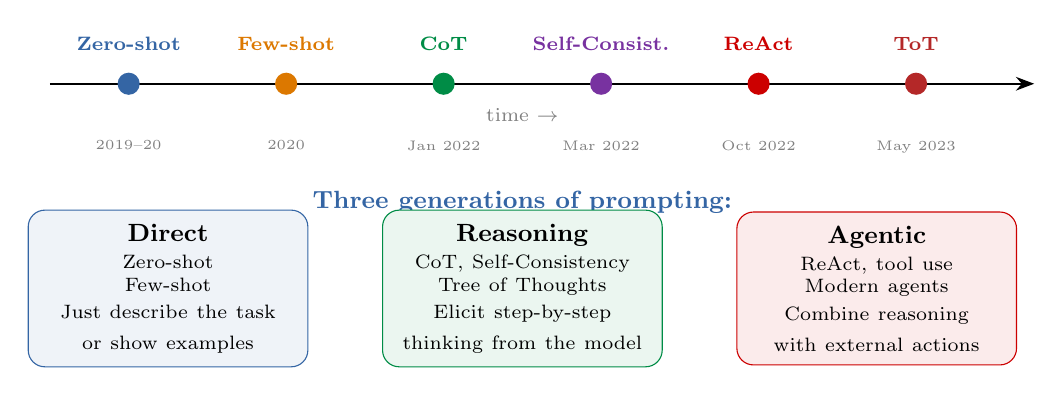
\begin{tikzpicture}
  % Timeline
  \draw[thick, -Stealth] (-6, 0) -- (6.5, 0);
  \node[font=\scriptsize, text=gray] at (0, -0.4) {time $\to$};

  % Zero-shot
  \fill[popblue] (-5, 0) circle (4pt);
  \node[font=\scriptsize\bfseries, text=popblue, above] at (-5, 0.3) {Zero-shot};
  \node[font=\tiny, text=gray, below] at (-5, -0.6) {2019--20};

  % Few-shot
  \fill[orange1] (-3, 0) circle (4pt);
  \node[font=\scriptsize\bfseries, text=orange1, above] at (-3, 0.3) {Few-shot};
  \node[font=\tiny, text=gray, below] at (-3, -0.6) {2020};

  % CoT
  \fill[paramgreen] (-1, 0) circle (4pt);
  \node[font=\scriptsize\bfseries, text=paramgreen, above] at (-1, 0.3) {CoT};
  \node[font=\tiny, text=gray, below] at (-1, -0.6) {Jan 2022};

  % Self-consistency / Zero-shot CoT
  \fill[violet1] (1, 0) circle (4pt);
  \node[font=\scriptsize\bfseries, text=violet1, above] at (1, 0.3) {Self-Consist.};
  \node[font=\tiny, text=gray, below] at (1, -0.6) {Mar 2022};

  % ReAct
  \fill[sampred] (3, 0) circle (4pt);
  \node[font=\scriptsize\bfseries, text=sampred, above] at (3, 0.3) {ReAct};
  \node[font=\tiny, text=gray, below] at (3, -0.6) {Oct 2022};

  % ToT
  \fill[warnred] (5, 0) circle (4pt);
  \node[font=\scriptsize\bfseries, text=warnred, above] at (5, 0.3) {ToT};
  \node[font=\tiny, text=gray, below] at (5, -0.6) {May 2023};

  % Categorization below
  \node[font=\small\bfseries, text=popblue] at (0, -1.5) {Three generations of prompting:};

  \node[draw=popblue, fill=popblue!8, rounded corners=6pt, text width=3.2cm, align=center, inner sep=5pt, font=\small] at (-4.5, -2.6) {
    \textbf{Direct}\\[2pt]
    {\scriptsize Zero-shot\\Few-shot\\[2pt]
    Just describe the task\\or show examples}
  };

  \node[draw=paramgreen, fill=paramgreen!8, rounded corners=6pt, text width=3.2cm, align=center, inner sep=5pt, font=\small] at (0, -2.6) {
    \textbf{Reasoning}\\[2pt]
    {\scriptsize CoT, Self-Consistency\\Tree of Thoughts\\[2pt]
    Elicit step-by-step\\thinking from the model}
  };

  \node[draw=sampred, fill=sampred!8, rounded corners=6pt, text width=3.2cm, align=center, inner sep=5pt, font=\small] at (4.5, -2.6) {
    \textbf{Agentic}\\[2pt]
    {\scriptsize ReAct, tool use\\Modern agents\\[2pt]
    Combine reasoning\\with external actions}
  };
\end{tikzpicture}
\end{center}
\end{frame}

% ============================================================
% COMPARISON TABLE
% ============================================================
\begin{frame}
\frametitle{Prompting techniques compared}

\vspace{-0.1cm}
\renewcommand{\arraystretch}{1.3}
\begin{center}
{\scriptsize
\begin{tabular}{l c c c c}
  \textbf{Technique} & \textbf{Examples needed} & \textbf{LLM calls} & \textbf{Best for} & \textbf{Key paper} \\
  \hline
  Zero-shot & None & 1 & Simple, common tasks & Radford 2019 \\[1pt]
  Few-shot & 2--5 demos & 1 & Format-sensitive tasks & Brown 2020 \\[1pt]
  Chain-of-Thought & Reasoning chains & 1 & Math, logic, multi-step & Wei 2022 \\[1pt]
  Zero-shot CoT & None (``step by step'') & 1 & Quick reasoning boost & Kojima 2022 \\[1pt]
  Self-Consistency & Reasoning chains & $N$ (5--40) & Verifiable answers & Wang 2022 \\[1pt]
  Tree of Thoughts & Task-specific & Many & Search/planning problems & Yao 2023 \\[1pt]
  ReAct & 1--2 demos & Multiple & Knowledge-grounded QA & Yao 2022 \\
  \hline
\end{tabular}
}
\end{center}

\vspace{0.2cm}
\begin{center}
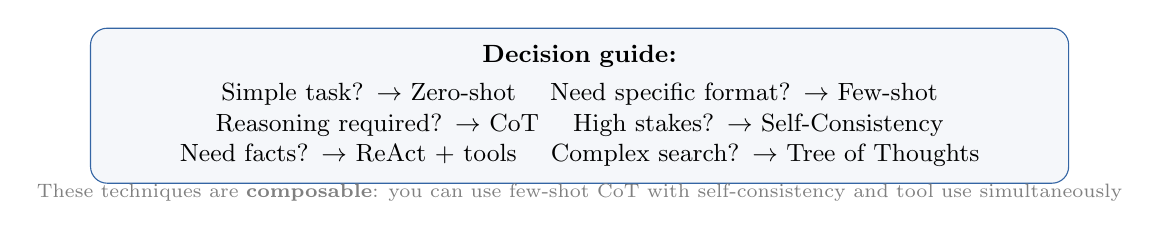
\begin{tikzpicture}
  \node[draw=popblue, fill=popblue!5, rounded corners=6pt, text width=12cm, align=center, inner sep=6pt, font=\small] at (0, 0.3) {
    \textbf{Decision guide:}\\[3pt]
    Simple task? $\to$ Zero-shot \quad
    Need specific format? $\to$ Few-shot\\
    Reasoning required? $\to$ CoT \quad
    High stakes? $\to$ Self-Consistency\\
    Need facts? $\to$ ReAct + tools \quad
    Complex search? $\to$ Tree of Thoughts
  };

  \node[font=\scriptsize, text=gray] at (0, -0.8) {
    These techniques are \textbf{composable}: you can use few-shot CoT with self-consistency and tool use simultaneously
  };
\end{tikzpicture}
\end{center}
\end{frame}

% ============================================================
% PRACTICAL: PROMPT DESIGN WALKTHROUGH
% ============================================================
\begin{frame}
\frametitle{Practical: designing a prompt step by step}

\begin{center}
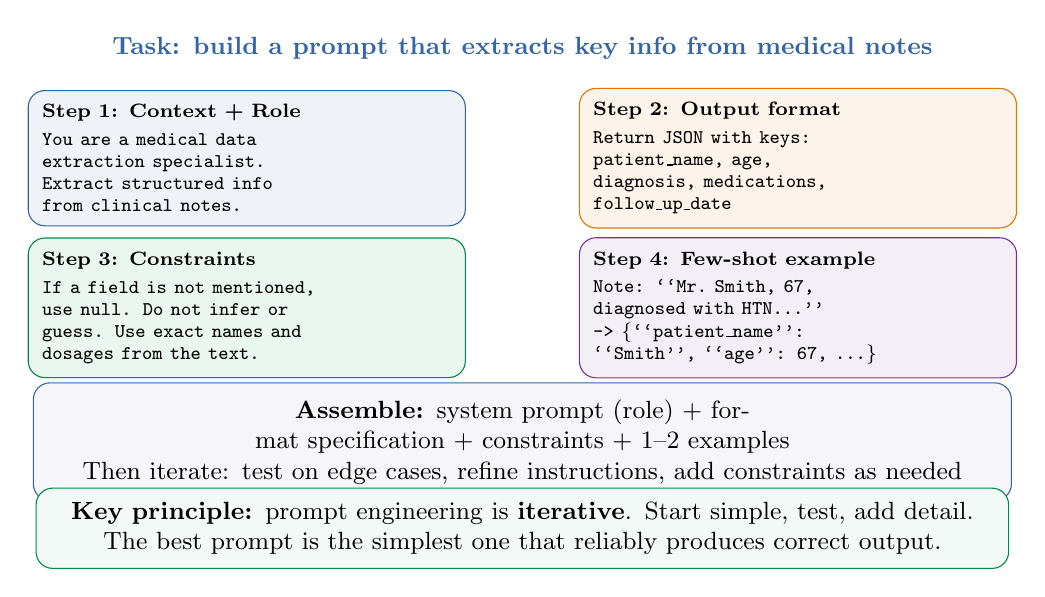
\begin{tikzpicture}
  \node[font=\small\bfseries, text=popblue] at (0, 3.2) {Task: build a prompt that extracts key info from medical notes};

  % Step 1
  \node[draw=popblue, fill=popblue!8, rounded corners=6pt, text width=5.2cm, align=left, inner sep=5pt, font=\scriptsize] at (-3.5, 1.8) {
    \textbf{Step 1: Context + Role}\\[2pt]
    \texttt{You are a medical data}\\
    \texttt{extraction specialist.}\\
    \texttt{Extract structured info}\\
    \texttt{from clinical notes.}
  };

  % Step 2
  \node[draw=orange1, fill=orange1!8, rounded corners=6pt, text width=5.2cm, align=left, inner sep=5pt, font=\scriptsize] at (3.5, 1.8) {
    \textbf{Step 2: Output format}\\[2pt]
    \texttt{Return JSON with keys:}\\
    \texttt{patient\_name, age,}\\
    \texttt{diagnosis, medications,}\\
    \texttt{follow\_up\_date}
  };

  % Step 3
  \node[draw=paramgreen, fill=paramgreen!8, rounded corners=6pt, text width=5.2cm, align=left, inner sep=5pt, font=\scriptsize] at (-3.5, -0.1) {
    \textbf{Step 3: Constraints}\\[2pt]
    \texttt{If a field is not mentioned,}\\
    \texttt{use null. Do not infer or}\\
    \texttt{guess. Use exact names and}\\
    \texttt{dosages from the text.}
  };

  % Step 4
  \node[draw=violet1, fill=violet1!8, rounded corners=6pt, text width=5.2cm, align=left, inner sep=5pt, font=\scriptsize] at (3.5, -0.1) {
    \textbf{Step 4: Few-shot example}\\[2pt]
    \texttt{Note: ``Mr.\ Smith, 67,}\\
    \texttt{diagnosed with HTN...''}\\
    \texttt{-> \{``patient\_name'':}\\
    \texttt{``Smith'', ``age'': 67, ...\}}
  };

  % Result
  \node[draw=popblue, fill=lightbg, rounded corners=6pt, text width=12cm, align=center, inner sep=6pt, font=\small] at (0, -1.8) {
    \textbf{Assemble:} system prompt (role) + format specification + constraints + 1--2 examples\\
    Then iterate: test on edge cases, refine instructions, add constraints as needed
  };

  \node[draw=paramgreen, fill=paramgreen!5, rounded corners=6pt, text width=12cm, align=center, inner sep=5pt, font=\small] at (0, -2.9) {
    \textbf{Key principle:} prompt engineering is \textbf{iterative}. Start simple, test, add detail.\\
    The best prompt is the simplest one that reliably produces correct output.
  };
\end{tikzpicture}
\end{center}
\end{frame}

% ============================================================
% QUESTIONS
% ============================================================
\begin{frame}
\begin{center}
\vspace{2cm}
{\Huge \textcolor{popblue}{Questions?}}

\vspace{1cm}
{\large Next: Hallucination \& Grounding}
\end{center}
\end{frame}

\end{document}
